
\textslideleft{

Cells accumulate information in a {\it bounded join-semilattice}

\pnl

A bounded join-semilattice is:

\begin{itemize}
\item A {\it partially ordered set}
\item with a least element
\item such that any subset of elements has a {\it least upper bound}
\end{itemize}

\pnl

``Least upper bound'' is denoted as $\vee$ and is usually pronounced ``join''

}

\begin{frame}
\begin{columns}
\column{0.7\textwidth}
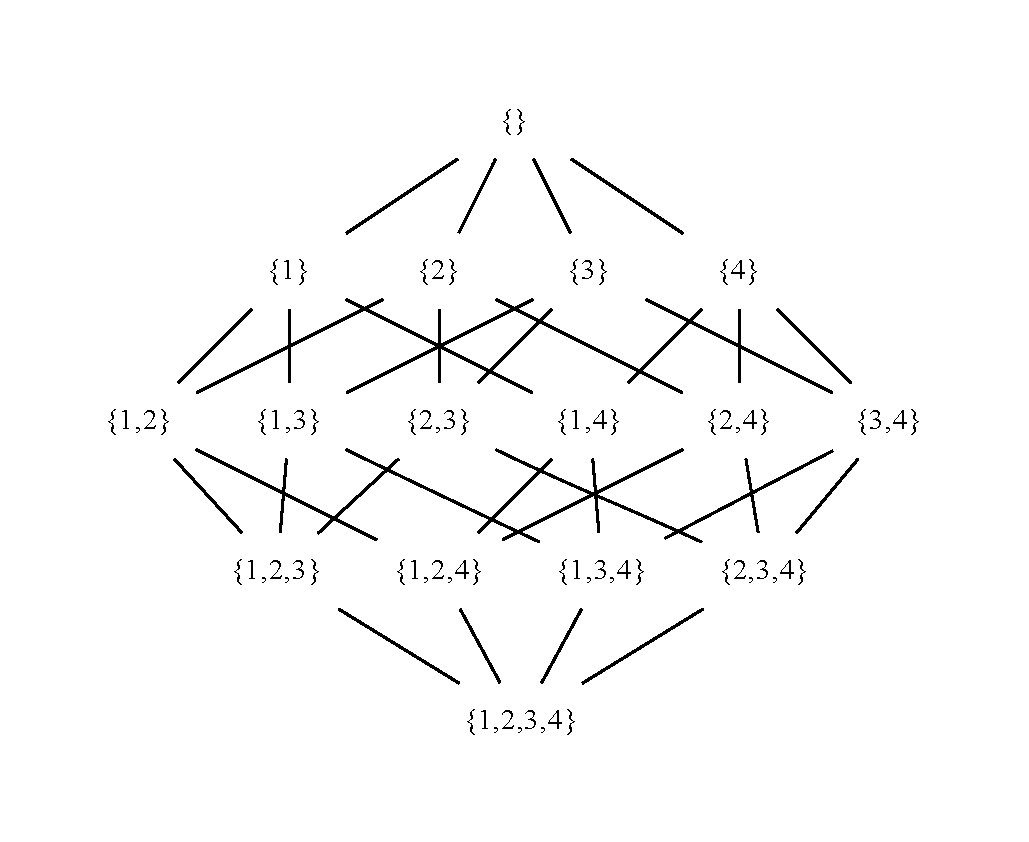
\includegraphics[scale=0.65]{powerset.pdf}
\pause
\column{0.3\textwidth}
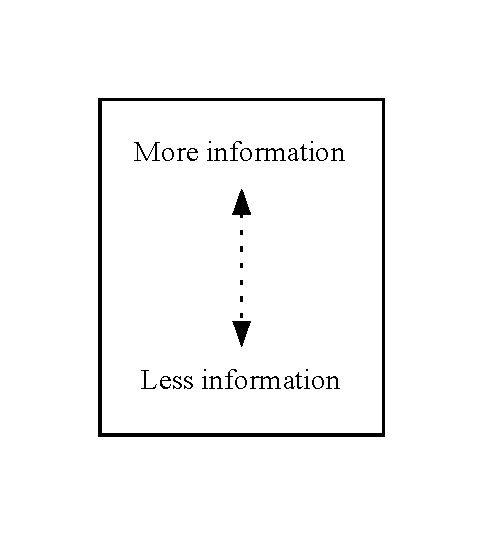
\includegraphics[scale=0.5]{more-information.pdf}
\end{columns}
\end{frame}


\latticeinfoslide{set/powerset-info1.pdf}
\latticeinfoslide{set/powerset-info2.pdf}
\latticeinfoslide{set/powerset-info3.pdf}
\latticeinfoslide{set/powerset-info4.pdf}

\latticeinfoslide{set/powerset1.pdf}
\latticeinfoslide{set/powerset2.pdf}
\latticeinfoslide{set/powerset3.pdf}
\latticeinfoslide{set/powerset4.pdf}
\latticeinfoslide{set/powerset5.pdf}
\latticeinfoslide{set/powerset6.pdf}

\textslideleft{
$\vee$ has useful algebraic properties. It is:

\begin{itemize}
\item A monoid
\item that's commutative
\item and idempotent
\end{itemize}
}

\textslide{
Left identity

$\epsilon \vee x = x$
\nl

Right identity

$x \vee \epsilon = x$
\nl

Associativity

$(x \vee y) \vee z = x \vee (y \vee z)$
\nl

Commutative

$x \vee y = y \vee x$
\nl

Idempotent

$x \vee x = x$
}

\begin{frame}[fragile]
  \begin{haskellcode}
class BoundedJoinSemilattice a where
  bottom :: a
  (\/) :: a -> a -> a
  \end{haskellcode}

  \pnl

  \begin{haskellcode}
data SudokuVal = One | Two | Three | Four
                 deriving (Eq, Ord, Show)
  \end{haskellcode}
  \pause
  \begin{haskellcode}
newtype SudokuSet = S (Set SudokuVal)
  \end{haskellcode}
  \pnl
  \begin{haskellcode}
instance BoundedJoinSemilattice SudokuSet where
  bottom     = S (Set.fromList [One, Two, Three, Four])
  S a \/ S b = S (Set.intersection a b)
  \end{haskellcode}
\end{frame}

\textslideleft{
  We don't write values directly to cells

  Instead we {\it join information in}

  \pnl

  This makes our propagators {\it monotone}, meaning that as the input cells gain information, the output cells gain information (or don't change)

  \pnl

  A function $f : A \rightarrow B$ where $A$ and $B$ are partially ordered sets is {\bf monotone} if and only if, \\
  for all $x,y \in A .$ $x \leq y \implies f(x) \leq f(y)$
}

\textslide{
  All our lattices so far have been fininte

  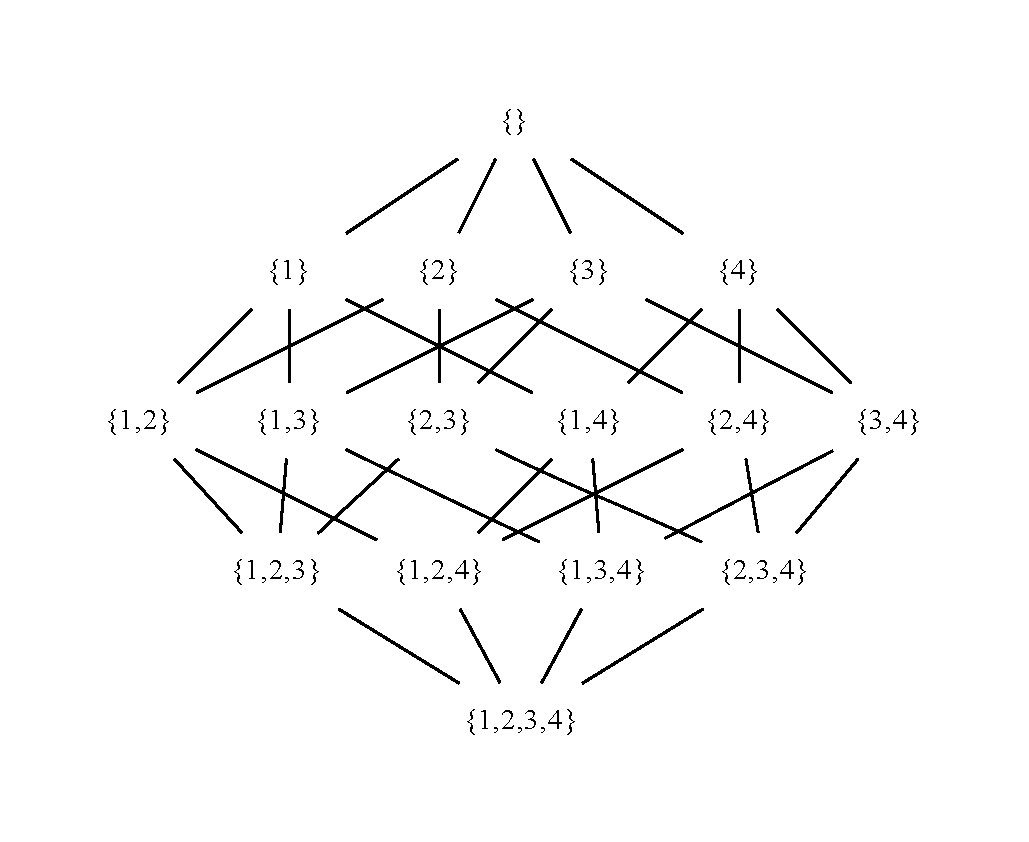
\includegraphics[scale=0.6]{powerset.pdf}
}

\textslideleft{
  Thanks to these properties:
  \begin{itemize}
    \item the bounded join-semilattice laws
    \item the finiteness of our lattice
    \item the monotonicity of our propagators
  \end{itemize}
  our propagator networks will yield with a deterministic answer, in finite time, regardless of parallelism and distribution

  \pnl

  Bounded join-semilattices are already popular in the distributed systems world

  See: Conflict Free Replicated Datatypes

  \pnl

  We can relax these constraints in a few different directions
}

\textslide{
  Our lattices only need the {\it ascending chain condition}

  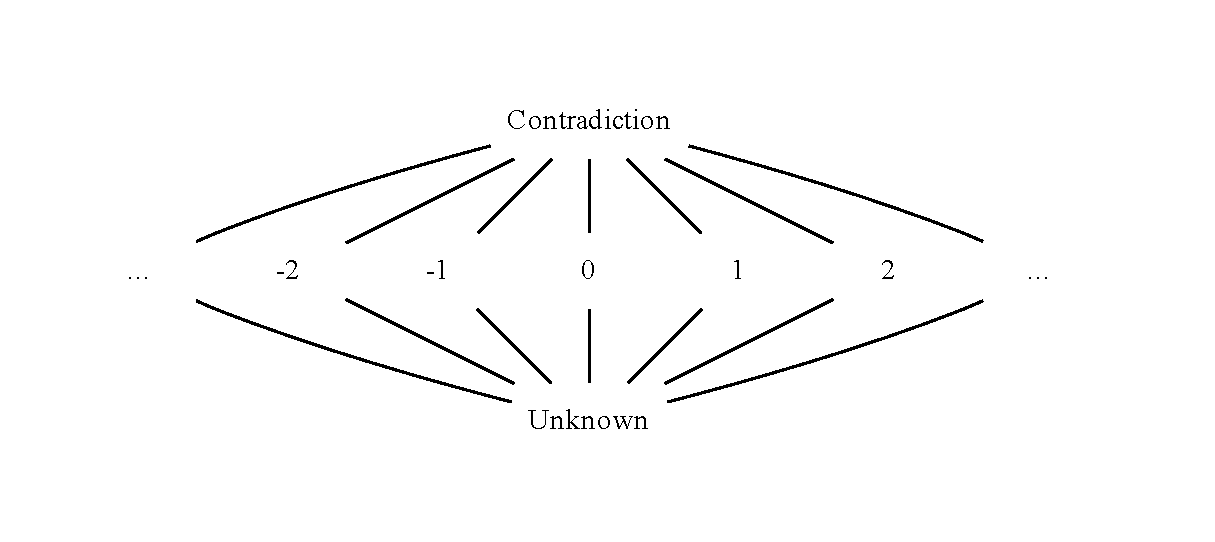
\includegraphics[scale=0.8]{flat.pdf}
}

\textslide{\Huge{?}}